\documentclass[12pt]{article}
\usepackage{fullpage}
\usepackage[normalem]{ulem}
\usepackage{fancyhdr,graphicx,amsmath,amssymb, mathtools, scrextend, titlesec, enumitem}
\usepackage[ruled,vlined]{algorithm2e} 
\usepackage{listings}
\usepackage{mathtools}
\usepackage{subcaption}
\usepackage{float}
\usepackage{bm}
\DeclarePairedDelimiter{\norm}{\lVert}{\rVert}
\DeclarePairedDelimiter{\abs}{\lvert}{\rvert}

\title{4M17 Coursework \#2: Practical Optimisation}
\author{CCN: \textbf{5673D}}
\begin{document}
\maketitle

\begin{enumerate}
	\item \textbf{Simulated Annealing}
	\begin{enumerate}
	\item \textbf{Problem-Specific Implementation Details}
	\begin{itemize}
		\item The specific implementation of simulated annealing used for this problem followed many of the suggestions in the 4M17 Simulated Annealing notes and was coded by myself in Python3. The full source code, along with comments, can be found in the Appendix. With regards to specific details, in some cases in the notes there were multiple suggestions as to best practice. With this in mind, I've implemented a few methods (and will evaluate them in more detail in a future section).
		\item \textbf{Burn-In}: I implemented a 'burn-in' period where I randomly sampled the function for a few iterations. I chose my start point $x_{\text{init}}$ to be the best random $x$ that resulted in the lowest objective function evaluation. 
		\item Moreover, I also used these results to form the basis of my \textbf{Initial Temperature}. I explored both using the standard deviation of objective function differences and also setting the temperature such that the probability of accepting an increase in objective function increase was $\bm{P}_{\text{init}}$.
		\item \textbf{Solution Generation}: New solutions were generated using the method suggested by Parks (1990) and the control variables $x$ were scaled to be in the range of (-1, 1). Alternative methods such as using the constant diagonal matrix $\bm{C}$ were also implemented. However, the method by Vanderbilt (1984) was not implemented owing to the need to use Cholesky decomposition, as well as the additional difficulty of calculating $\bm{X}$.
		\item \textbf{Constraints}: The nature of the task defined limits on the control variables such that $abs(x_{i}) \leq 512$ for every dimension. These constraints were handled by clipping values of $\bm{x}$ that left the bounded region. I also investigated with an alternative mechanism where I would ignore any generated point outside the problem bounds and would instead re-generate the control variable. This method didn't yield as strong a result (across both the 2D and 5D case - irrespective of the algorithm used).
		\item \textbf{Solution Assessment}: The probability of accepting a solution is as in the notes. Two different methods were used to calculate $p$ - depending on the nature of the process used for Solution Generation (i.e. when using Parks' method, there is an additional $\bar{d}$ term on the denominator in the exponent).
		\item \textbf{Temperature Decrement}: Temperatures were decremented in two ways: either with the simple exponential cooling scheme or with the adaptive annealing schedule proposed by Huang (1996).
		\item \textbf{Final Temperature}: The search is halted with the enhanced method in the notes: when there is no improvement in the global solution over the entire Markov Chain and the acceptance ratio falls below a threshold value $\bm{\chi_{f}}$). A hard cut=off was also placed when 10000 objective function evaluations had occurred, as specified by the task. 
		\item \textbf{Other}: Restarts were also implemented although there was no need for them in the 2D Eggholder case. Finally, \textbf{Markov Chain lengths} $L_{k}$ were chosen such that there could be a large number of chains within the 10000 objective function evaluation limits.
	\end{itemize}
	\item \textbf{Evaluation on 2D Eggholder Function}
	\begin{itemize}
		\item To demonstrate that Simulated Annealing is working, I ran my vanilla implementation on the 2D Eggholder function and, after 50 runs, the minimum objective function was determined to be $-959.6406600$ at $[512, 404.23025855]$. In every case, the algorithm terminates far before performing 10000 objective function evaluations (the maximum allowable limit).
		\item This value is very close (within $< 0.001\%$ error) to the true global minima in this region (listed online as $−959.6406627$).
		\item In addition, it's also necessary to show that the walks that Simulated Annealing go through at a given temperature are also reasonable. With this in mind, it is clear from Figure \ref{fig1} that the algorithms' walks are sensible; Initially, when the temperature is high, the walk traverses the entire state-space in a seemingly random manner (which makes sense as all updates will be accepted)
		\item However, as the temperature lowers, the walks become less random/dense and begin to converge to a localised area. At the lowest temperature, the walk traverses only  around the local minimum as in Figure \ref{fig1}d. In this case, the local minimum is in fact global minimum although this isn't necessarily always the case. 
		\item In the case of the 2D Eggholder, the algorithm overwhelmingly terminates at the global minimum.
		\item Another way of evaluating the algorithm is through determining the distribution of minima the algorithm terminates at. This was achieved by running the algorithm through multiple runs (i.e. 100) and binning minima into square regions of length 10. 
		\item Figure \ref{fig2} shows the histogram for these regions: with the most probable top two regions being in the immediate area around the true global minimum with a similar mean objective function value (note the $x_{2}$ values is $404$ and this will be split between the $400$ and $410$ bins. 
		\item The slight discrepancy between the 'global minimum' mean f(x) values and that of the true global minimum is likely because the algorithm likely terminates close to but not necessarily at the global minimum from run-to-run.
		\item Finally Figure \ref{fig4} shows the typical change in the objective function with the \# of iterations. The trend is generally decreasing: albeit with a lot of noise due to an initial high probability of acceptance as well as Markov Chain resets. This indicates that the SA algorithm is working well and Figure \ref{fig3} aptly shows that the algorithm does explore the state-space properly.
		\begin{figure}[ht]
		\centering
		\begin{subfigure}{8cm}
		\centering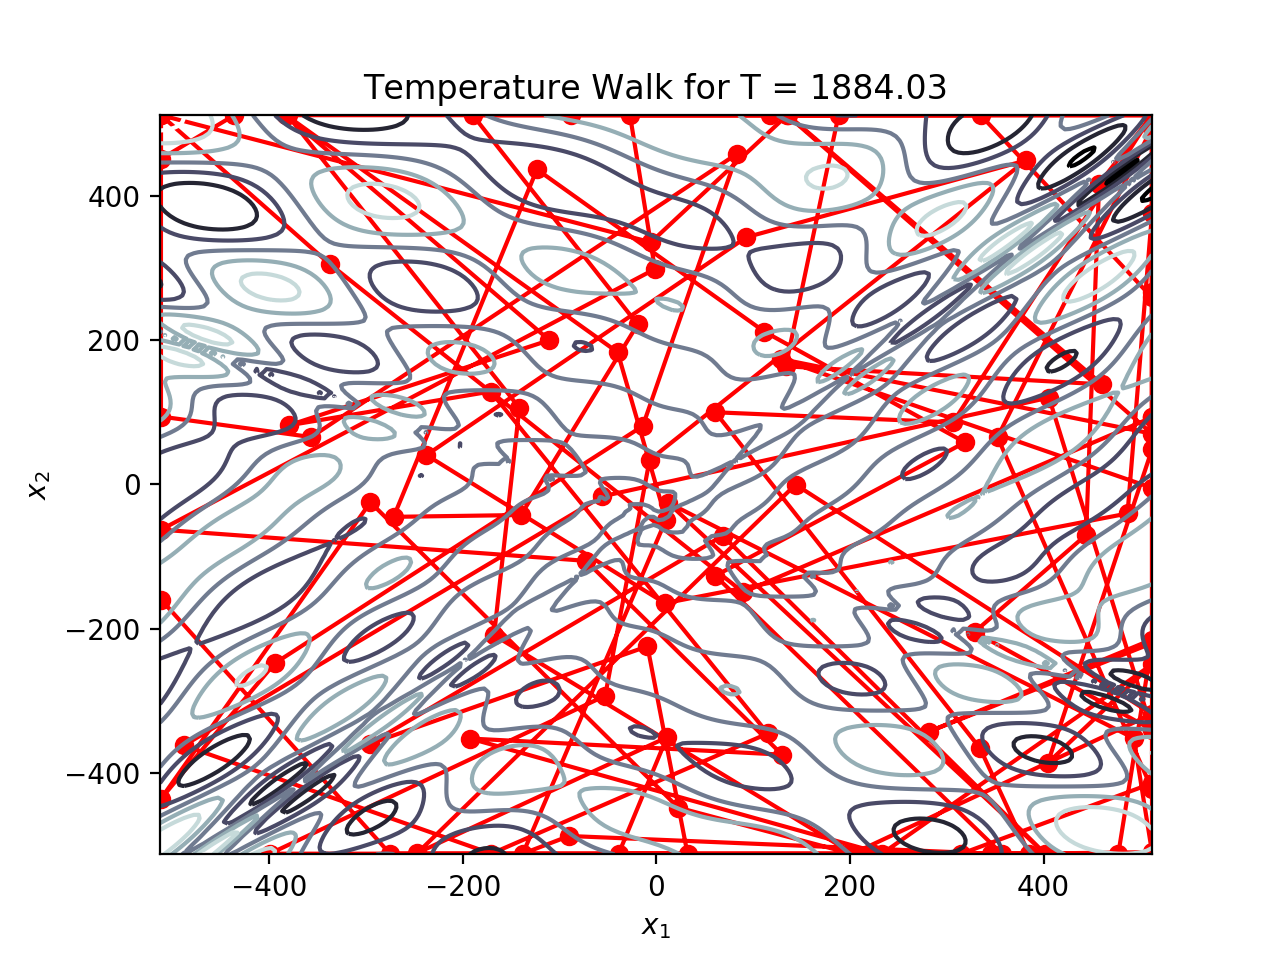
\includegraphics[width=8cm]{a_T_1}
		\caption{Temperature: 1884.03}
		\end{subfigure}%
		\begin{subfigure}{8cm}
		\centering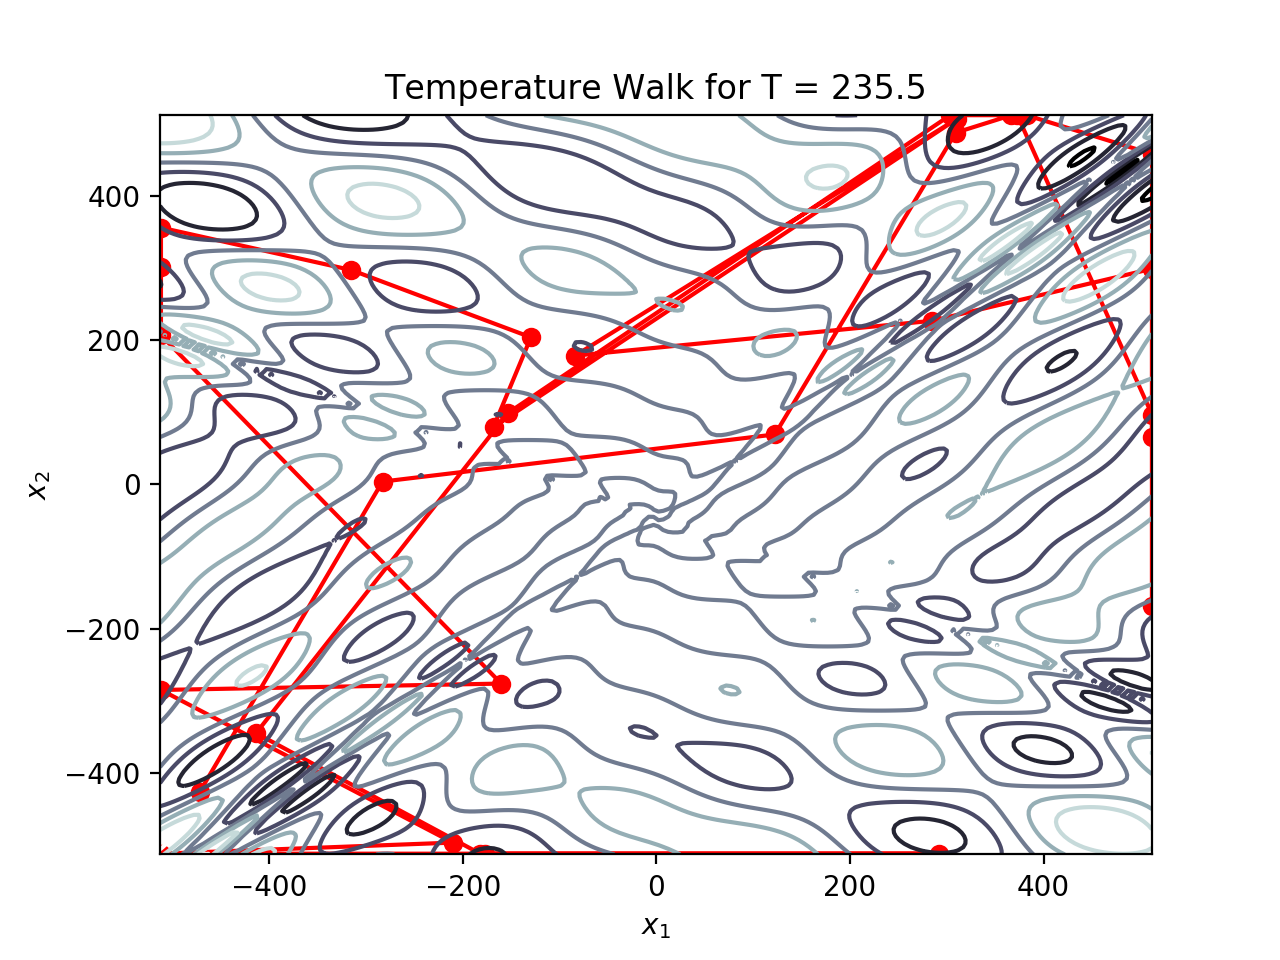
\includegraphics[width=8cm]{a_T_2}
		\caption{Temperature: 235.5}
		\end{subfigure}\vspace{10pt}
		\begin{subfigure}{8cm}
		\centering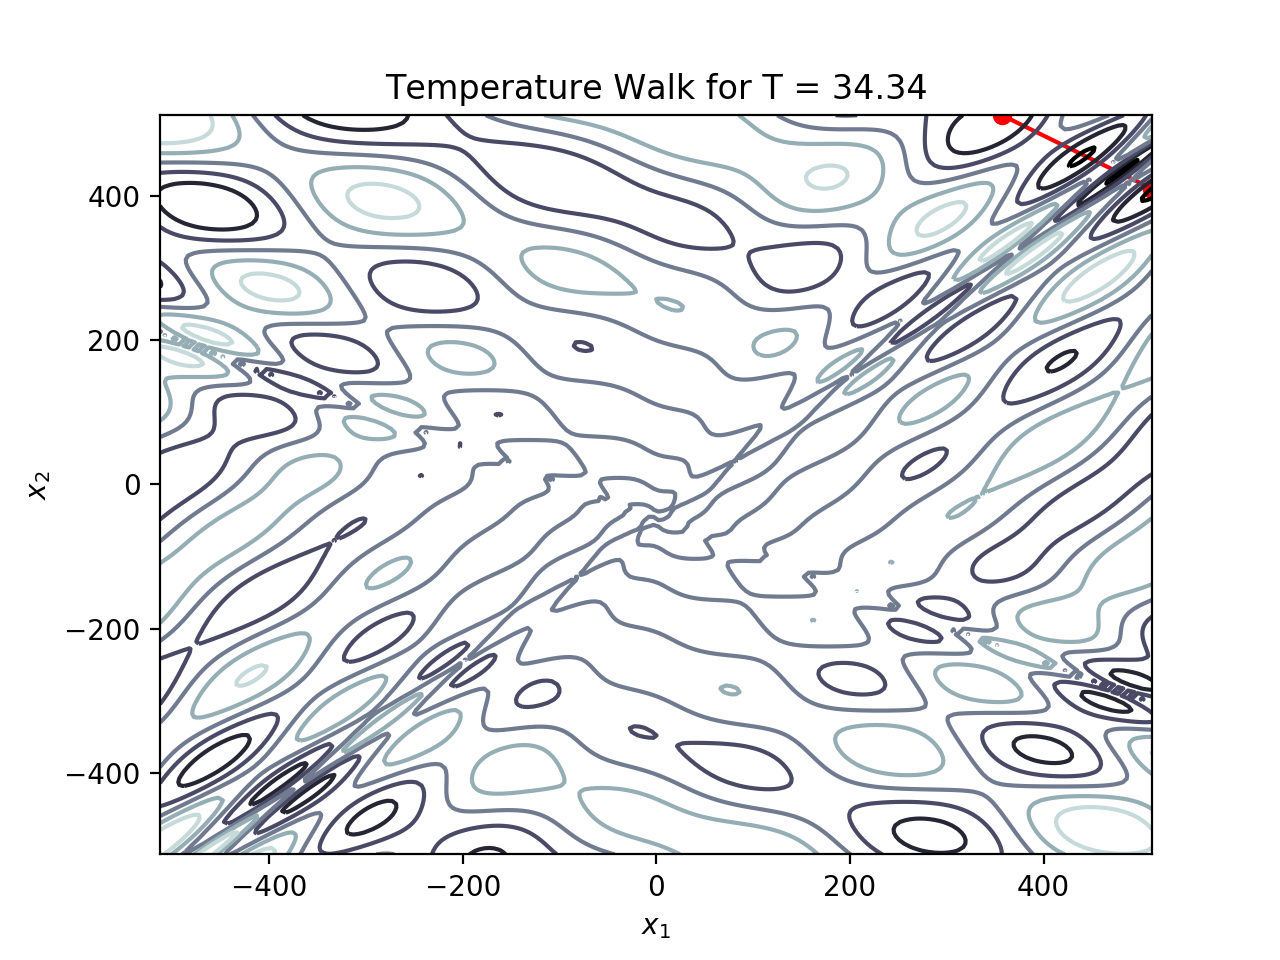
\includegraphics[width=8cm]{a_T_3}
		\caption{Temperature: 34.34}
		\end{subfigure}%
		\begin{subfigure}{8cm}
		\centering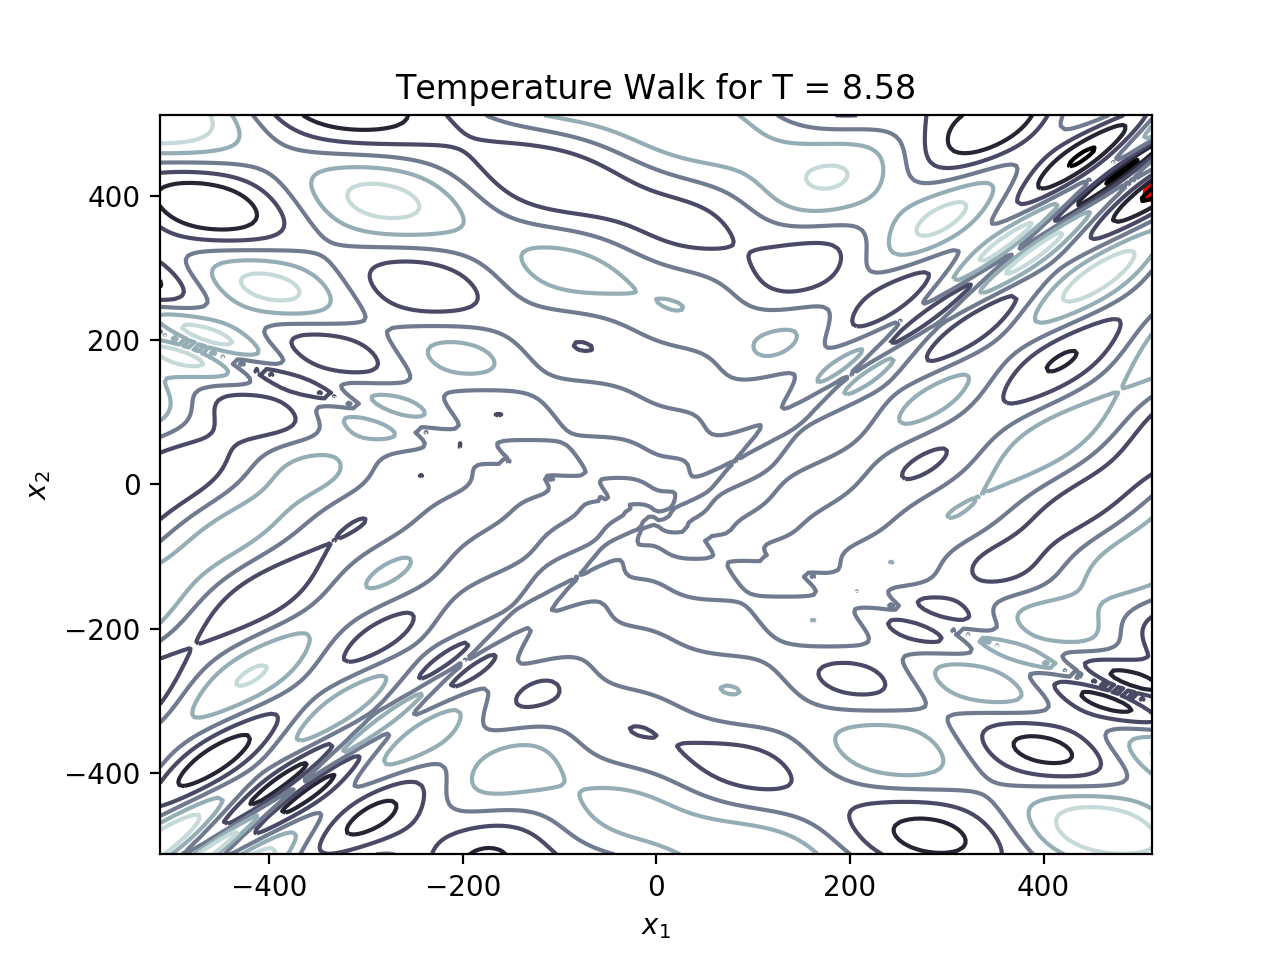
\includegraphics[width=8cm]{a_T_4}
		\caption{Temperature: 8.58}
		\end{subfigure}
		\caption{Simulated Annealing walk at different temperatures}
		\label{fig1}
		\end{figure}
		\begin{figure}[H]
		\centering
		\begin{subfigure}{8cm}
		\centering
		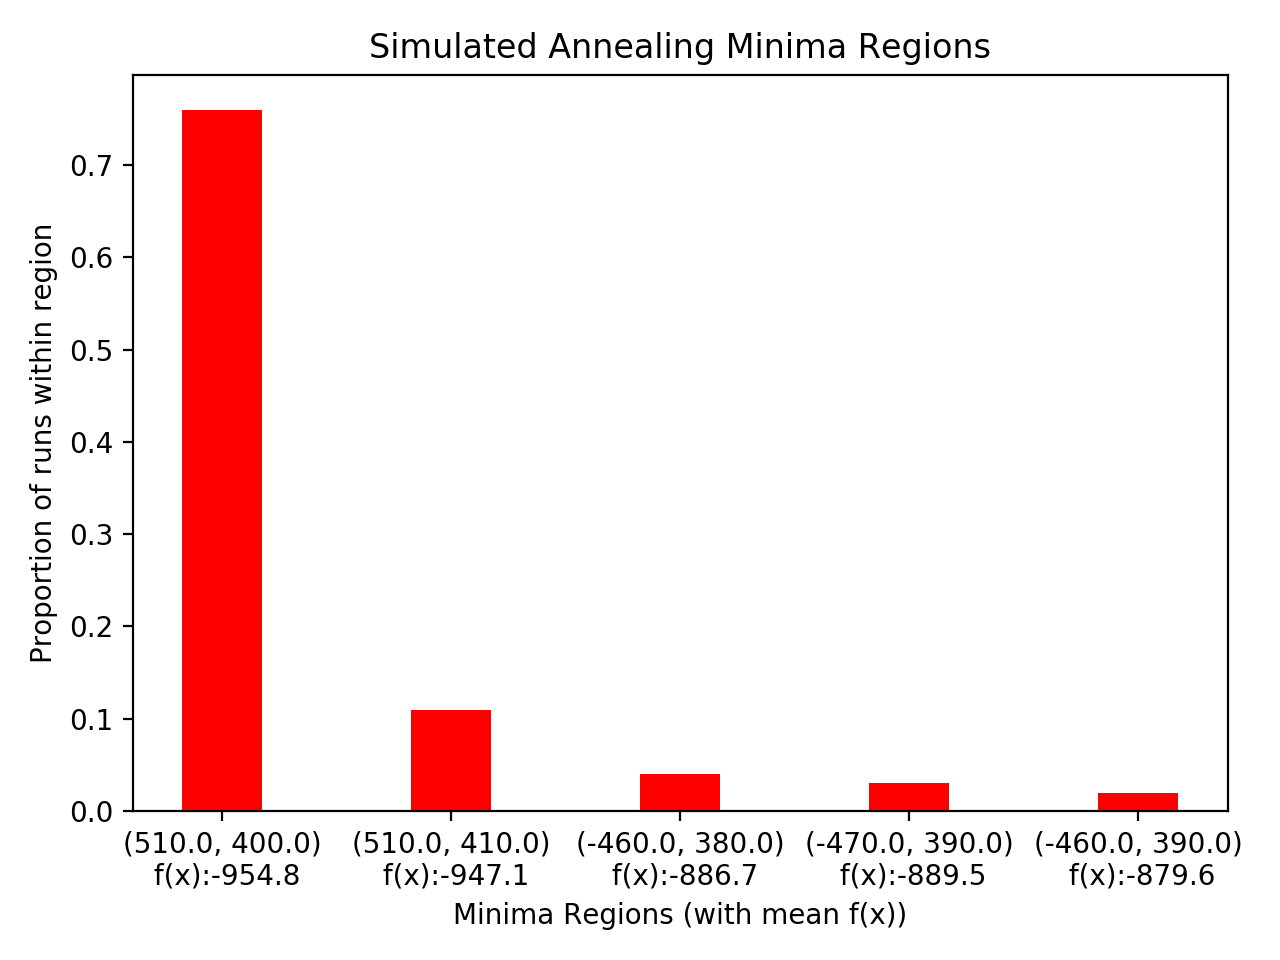
\includegraphics[width=8cm]{a_hist_bin}
		\caption{Histogram Regions}
		\end{subfigure}%
		\begin{subfigure}{8cm}
		\centering
		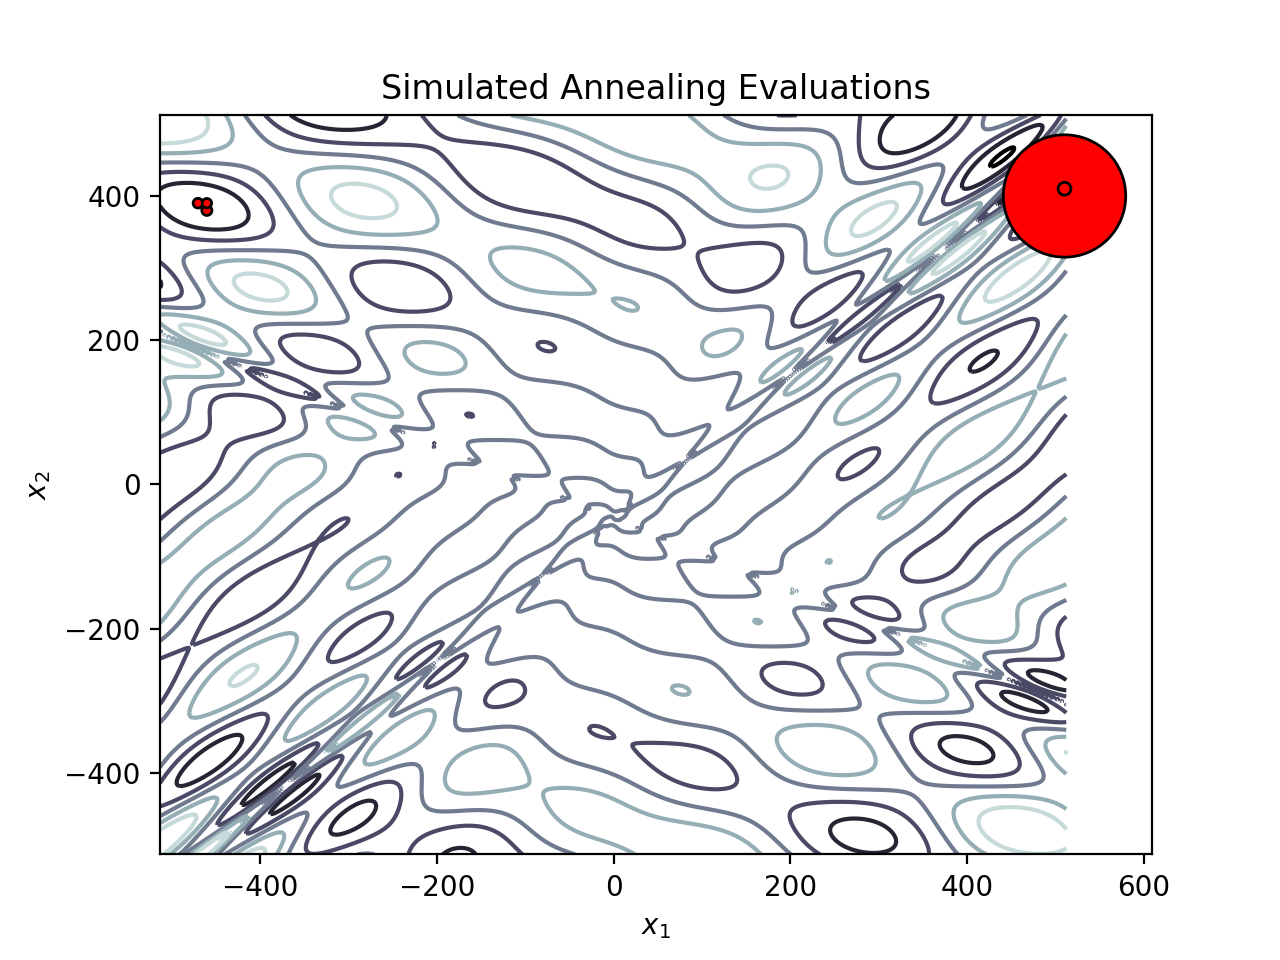
\includegraphics[width=8cm]{a_hist_plot}
		\caption{Regions on plot (with relative frequency)}
		\end{subfigure}
		\caption{Minima regions found after 100 iterations. Global minimum at $[512, 404]$}
		\label{fig2}
		\end{figure}
		\begin{figure}[H]
		\centering
		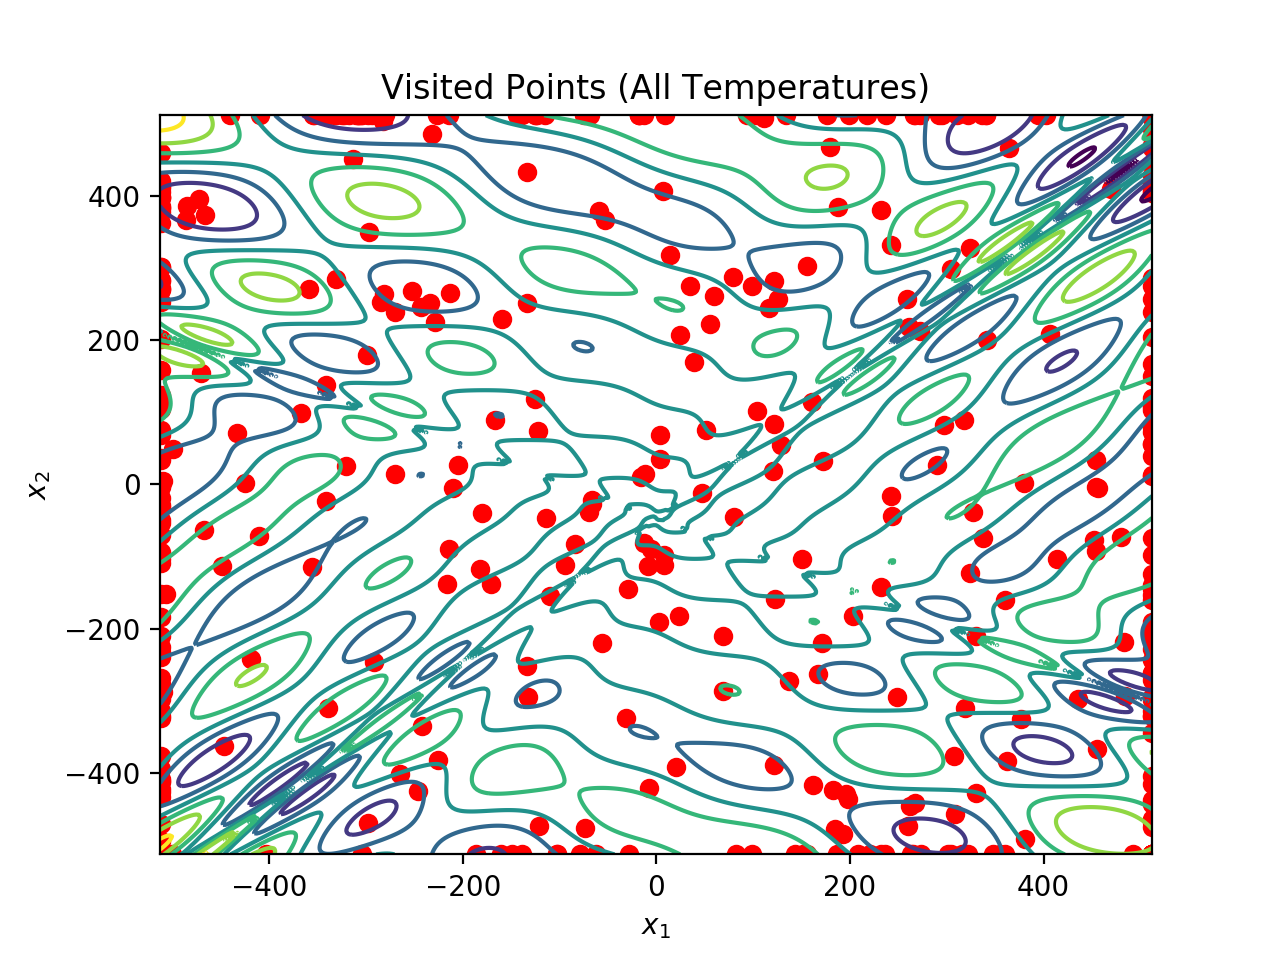
\includegraphics[width=\textwidth]{a_search_typical.png}
		\caption{A typical search pattern of a Simulated Annealing run}
		\label{fig3}
		\end{figure}
		\begin{figure}[H]
		\centering
		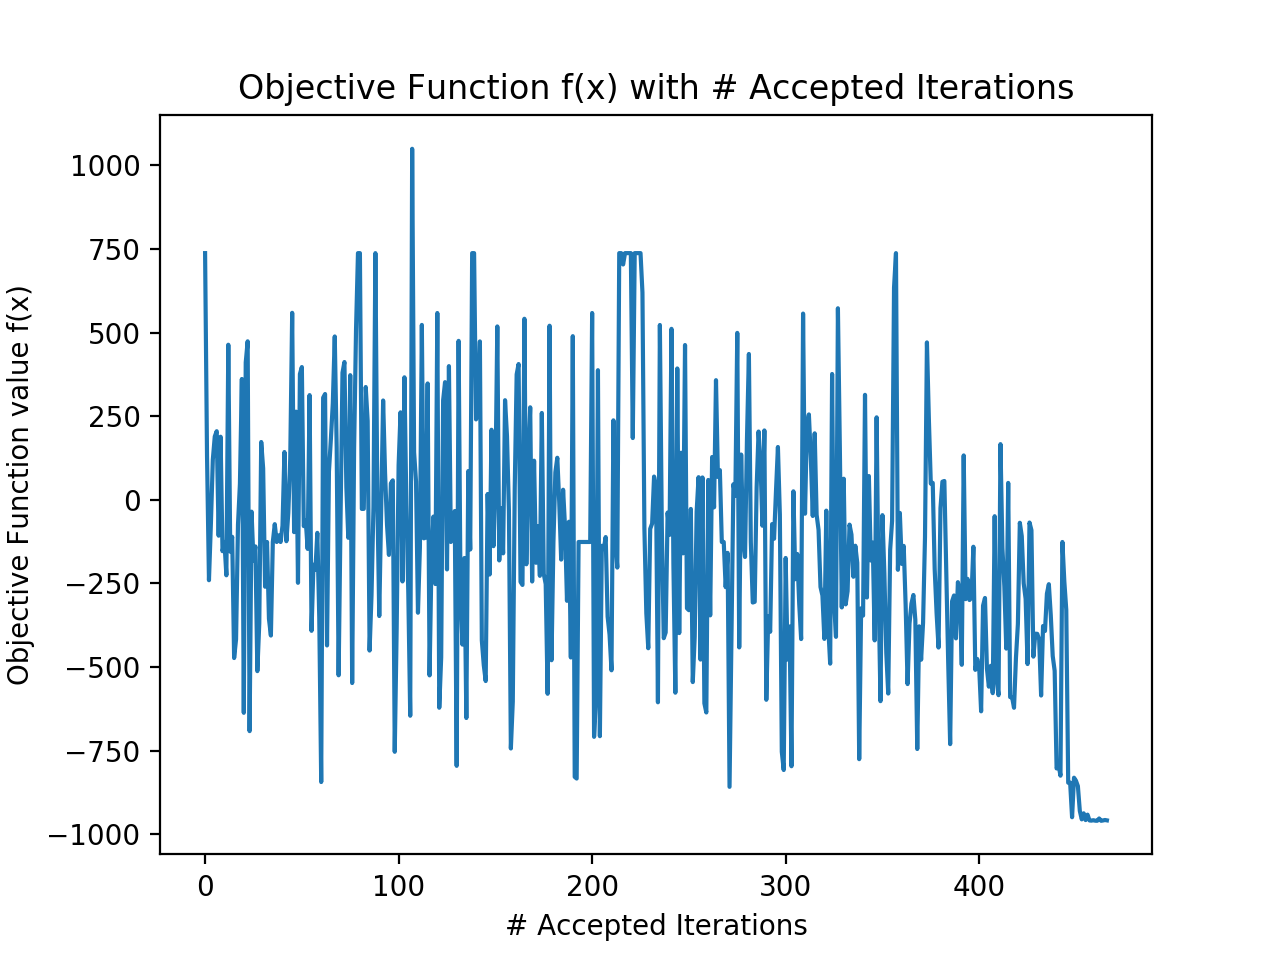
\includegraphics[width=\textwidth]{a_f_plot}
		\caption{A typical variation in objective function with \# accepted iterations}
		\label{fig4}
		\end{figure}

	\end{itemize}
	\item \textbf{Evaluation on 5D Eggholder Function}
	\begin{itemize}
		\item The 5D Eggholder Functions is a much more challenging problem than its 2D counterpart because there are far more local minima in the same range. As a result, parameters to control temperature annealing for example become far more important because they help to escape local minima. 
		\item In the 2D case, changing these parameters didn't really make much of a difference due to the limited size of the state-space. However, the 5D case is a $1024^5$-sized [continuous] state-space (as opposed to $1024^2$) and thus these parameters become a lot more important.
		\item Thus, the main body of this investigation will be focussed around looking at parameters and implementations that, when varied, will have the largest impact on minimising the objective function.
		\item In general the algorithm performed well although it found multiple areas where the objective function dropped below $-3000$ - indicating, as discussed, a large number of `good' local minima. The lowest recorded value was $-3424.05$ with the following $x$ coordinates: $[431.01,  441.1, 445.6,  453.2, 476.0]$.

		\item \textbf{Evaluating performance:}
		\begin{itemize}
			\item I evaluated the effectiveness of varying hyper-parameters/implementations within Simulated Annealing by observing both the minimum and average objective function values across $100$ runs with each implementation.
			\item Because the minimum overall objective function tends to be dependent on the initialisation of the control variables and thus is highly stochastic, for plots that weren't histograms, I decided to average the \textbf{top 25} values determined at each run as per the \textbf{Best L solutions} proposed in the notes. This process was used in all of the experiments below and is referred to as the 'average minimum objective function value'.
			\item A more complex system of \textbf{dissimilarity archiving} was also considered (as suggested in the notes to avoid just averaging results from the same funtion minimum).
			\item However, given the size of the state-space and the results that I observed, a dissimilarity archive was not required - especially given the large number of local minima in this problem. From my observations, there were very few duplicates in minima - even over $100$ runs.
		\end{itemize}
		\pagebreak
		\item \textbf{Temperature Cooling - Adaptive vs. ECS}:
		\begin{itemize}
		\item Firstly, the effectiveness of vanilla implementations of the Adaptive and Exponential Cooling Schemes were compared (using the hyper-parameters specified in the notes).
		\item The \textbf{simple ECS} had an average minimum objective function value $-2599.6$, with a standard deviation of $178.9$ and an overall minimum of $-3096.0$.
		\item Meanwhile, the \textbf{adaptive cooling} method proposed by Huang had an average of $-2679.7$, with a standard deviation of $202.3$ and an overall minimum of $-3174.7$.
		\item Figure \ref{fig5} corroborates these results (with another set of runs): the average minimum for adaptive cooling is indeed lower than that of ECS. However, it is necessary to note that this difference is on the order of $100$ which is small in the context of a minimum value in the thousands.
		\item By printing the true 'alpha' using adaptive cooling, the effective alpha values used in adaptive cooling are significantly smaller than the $0.95$ in ECS which means the decay in accepting increases in the objective function is much more significant. Thus, it is possible that adaptive cooling makes the function more likely to reach a local minimum and thus achieve a lower average objective function.
		\begin{figure}[H]
		\centering
		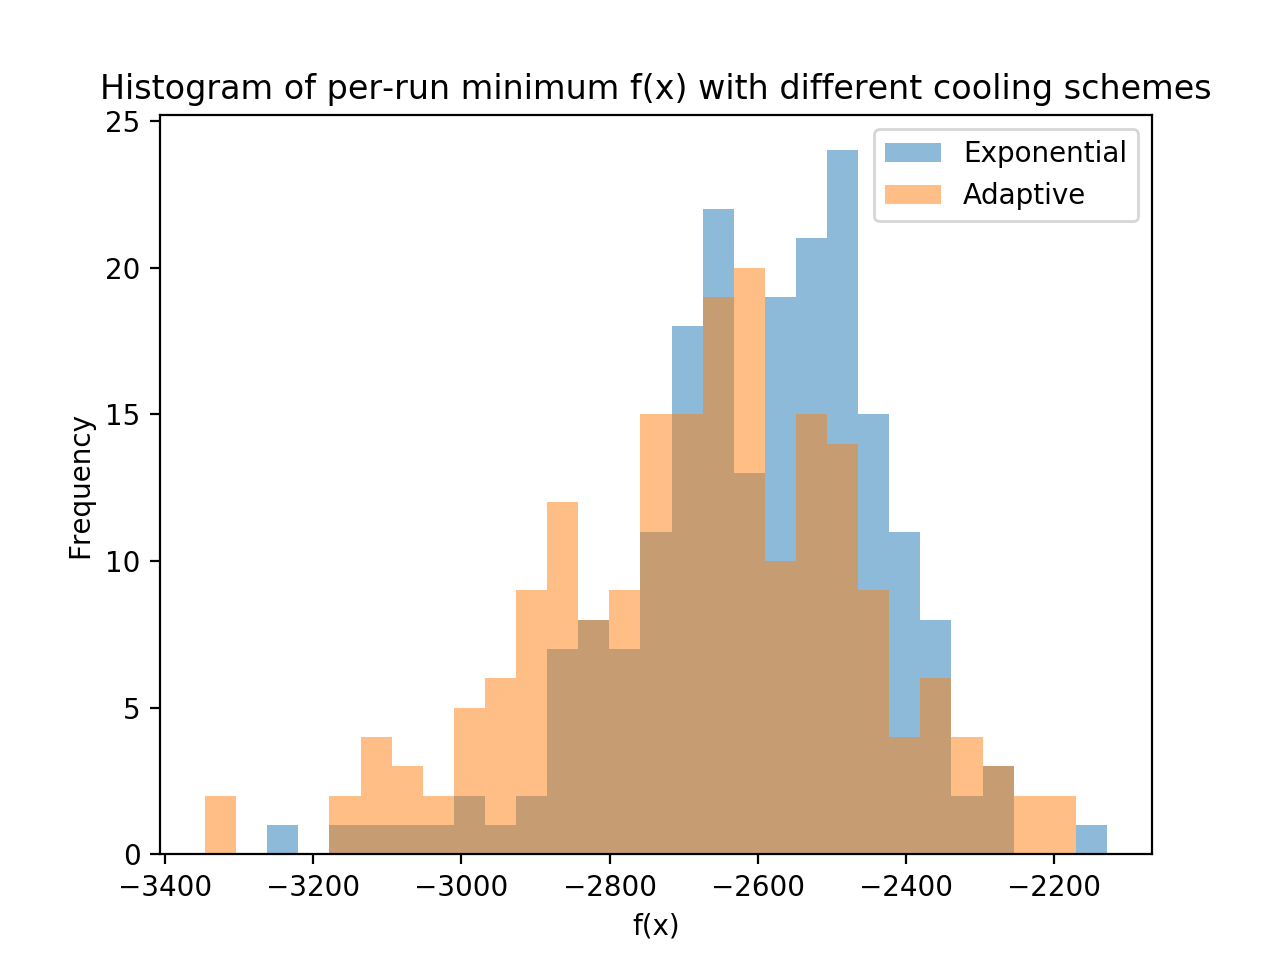
\includegraphics[width=11cm]{a_cooling_hist}
		\caption{Histogram of objective function between ECS and Adaptive cooling}
		\label{fig5}
		\end{figure}
		\end{itemize}
		\pagebreak
		\item \textbf{Exponential Cooling Scheme - Varying Alpha}
		\begin{itemize}
		\item Given the results from the previous experiment, I thought it would be worthwhile to explore varying the $a$ (alpha) parameter in ECS - to see if using a lower alpha would give results that are similar to those from Adaptive Cooling in Figure \ref{fig5}. 
		\item This was achieved by varying alpha from 0 to 1 at 20 evenly spaced values. The standard deviation and average minimum objective function values were recorded and plotted for each value of alpha and can be seen in Figure \ref{fig6} below.
		\item From the figure, varying the alpha parameter doesn't have a significant effect on the average minimum value although there is still a noticeable effect. Interestingly, this isn't the same for true minimum value found at each alpha - the value remained in the region of $-3100 - -3200$ with no noticeable pattern.
		\item Interestingly, alpha values close to 0 give a higher average minimum which makes sense as SA is most likely stuck at some non-optimal local minimum. Similarly, values of alpha near 1 seem to also give a high average minimum which also makes sense as SA is more likely to accept positive changes and thus may not reach a true local minimum. 
		\item An alpha value of $0.7$ seems to produce the lowest average minimum at $-2731$ which is similar to the value found through adaptive cooling (which also had an effective alpha value roughly in that region).
		\begin{figure}[H]
		\centering
		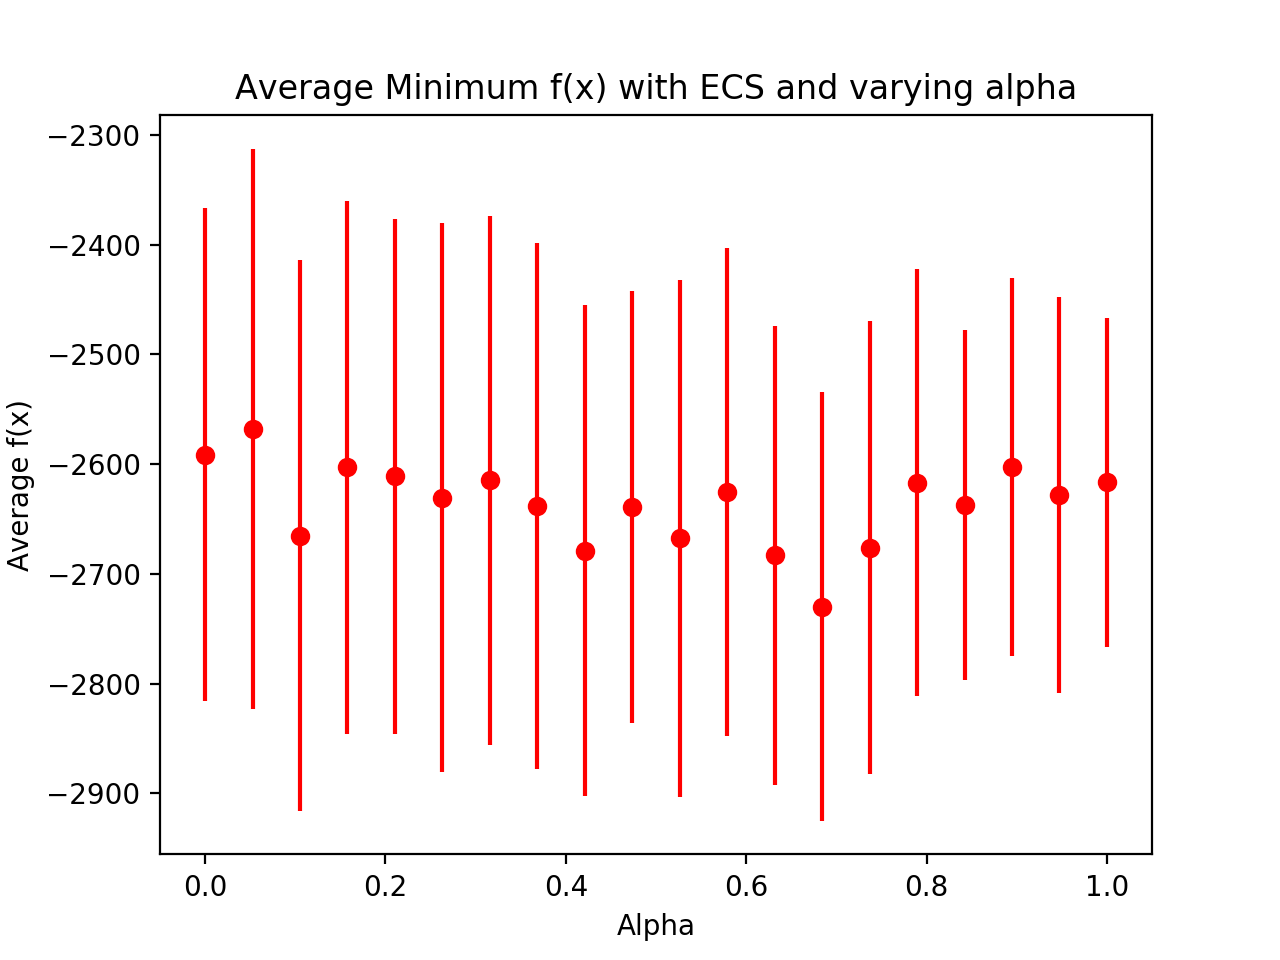
\includegraphics[width=12cm]{a_alpha_vary}
		\caption{Average objective function using ECS with varying alpha}
		\label{fig6}
		\end{figure}
		\end{itemize}
		\pagebreak
		\item \textbf{Parks' Update vs. Constant Update}	
		\begin{itemize}
		\item Given the substantial additional complexity in implementing the process developed by Parks, I wanted to understand its benefits over using a preset matrix $\bm{C}$ to generate the update on $x$. 
		\item Note, there is additional complexity here because there is a dependence on the magnitude of the $\bm{D}$ matrix, as well as the magnitude of $\bm{C}$ (both of which control the distance between consecutive control variables).
		\item To adjust for this, I chose the magnitude of each element in $\bm{C}$ to be 512 and each element in $\bm{D}$ to be initially 2. This means that the entire state space can be searched in both implementations (irrespective of $x_{\text{init}}$).
		\item The results were as follows: using SA with the simple constant $\bm{C}$ matrix gives an average minium objective function value of $-2584.7$ with a overall minimum of $-2994.1$ and a standard deviation of $166.4$. At the same time, the method by Parks' gives an average value of $-2646.7$ with a minimum value of $-3129.8$ and a standard deviation of $186.2$. 
		\item This indicates that the Parks method is performing slightly better - perhaps due to the fact that $\bm{D}$ is adaptive with every acceptance.
		\item Figure \ref{fig7} seems to also show that Parks' update method is performing better - with a slight shift in the histogram to a lower average f(x) (which indicates the algorithm is finding `better' minimums by better exploring the state-space). However, the data is slightly more spread apart in Parks' method (compared to the constant matrix) and this may be due to the effect of the variability of the $\bm{D}$ matrix' element magnitudes over time.	\begin{figure}[H]
		\centering
		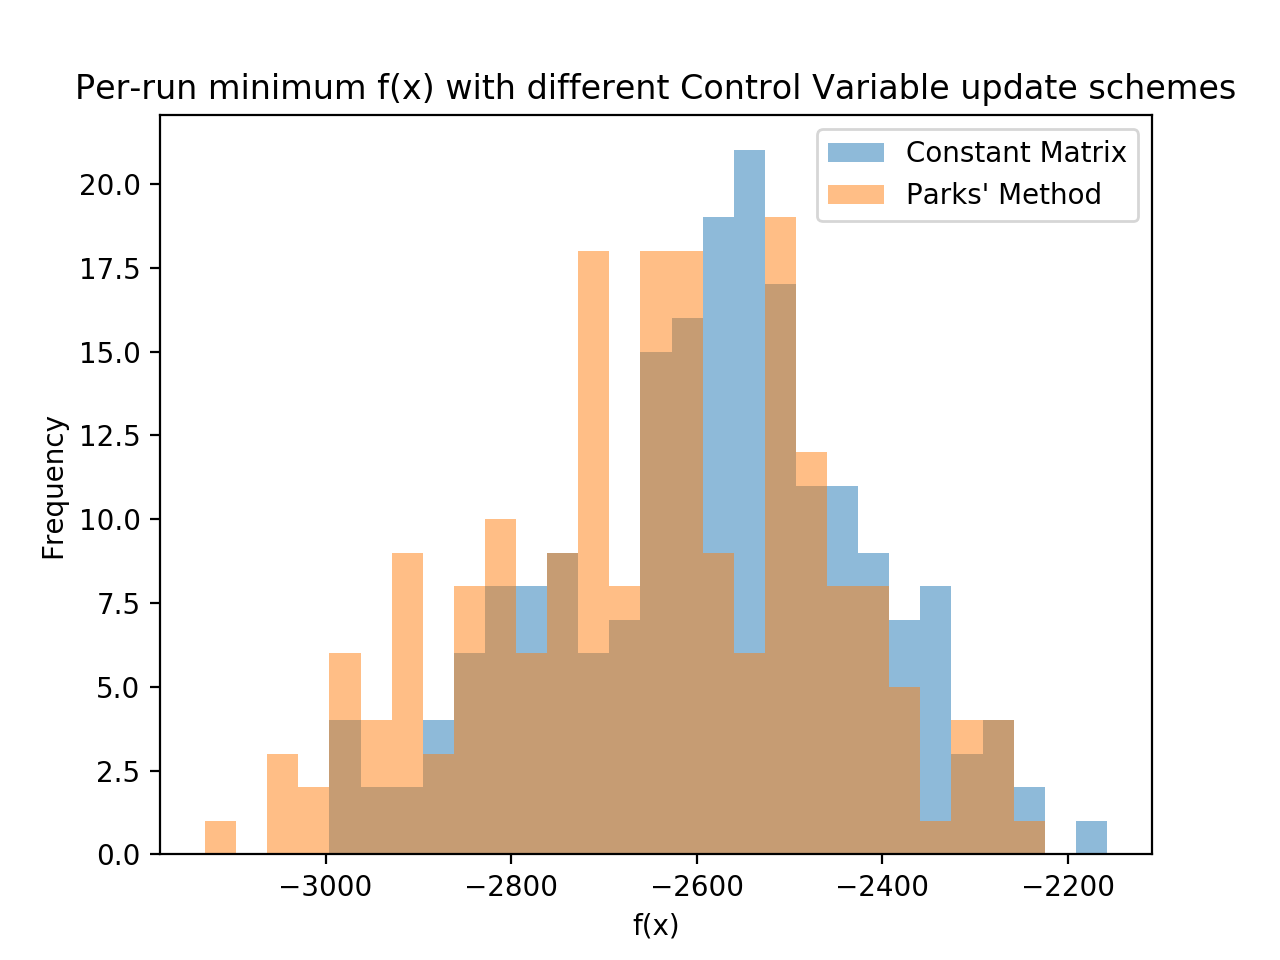
\includegraphics[width=11cm]{a_control_vars}
		\caption{Histogram of objective function with varying update schemes}
		\label{fig7}
		\end{figure}
		\end{itemize} 
		\pagebreak
		\item \textbf{Control Variables: Varying magnitude of elements in $\bm{D}$ \& ${\bm{C}}$}
		\begin{itemize}
		\item I also wanted to investigate the effect of varying the magnitude of each of the elements in $\bm{C}$ or $\bm{D}$. Note that in the case of Parks' method, the magnitudes of these elements would change with each successful solution acceptances - nevertheless the initial magnitude would serve as a 'seed' for future updates to the matrix.
		\item It is clear that varying the magnitude of these elements did not have a significant effect on the results. From Figure \ref{fig8}, there seems to be no clear pattern aside from a zero-magnitude matrix giving a poor result: this is expected as it essentially zeros out any update to $x$ and so the algorithm effectively acts as a random sampler. 
		\item That being said, the standard deviation of the local average minima does reduce with increasing magnitude in both cases - likely because local state-space effects are less influential. In addition, the higher the magnitude, the (slightly) higher the average minimum f(x) - which indicates the algorithm isn't performing as well.
		\item To fully verify these results are due to the vanilla SA implementation, I removed burn-in and re-ran the same tests. The trend observed (as in Figure \ref{fig8}) remained the same: this makes sense as I averaged my values over 25 runs and the burn-in period (which itself is random) would be different for each run.
		\item It can be concluded that as long as the magnitude is non-zero, the SA algorithm is able to suitably traverse the space irrespective of the control variable update matrix magnitude - although, smaller magnitudes seem to perform more reasonably. 
		\begin {figure}[H]
		\centering
		\begin{subfigure}{8cm}
		\centering
		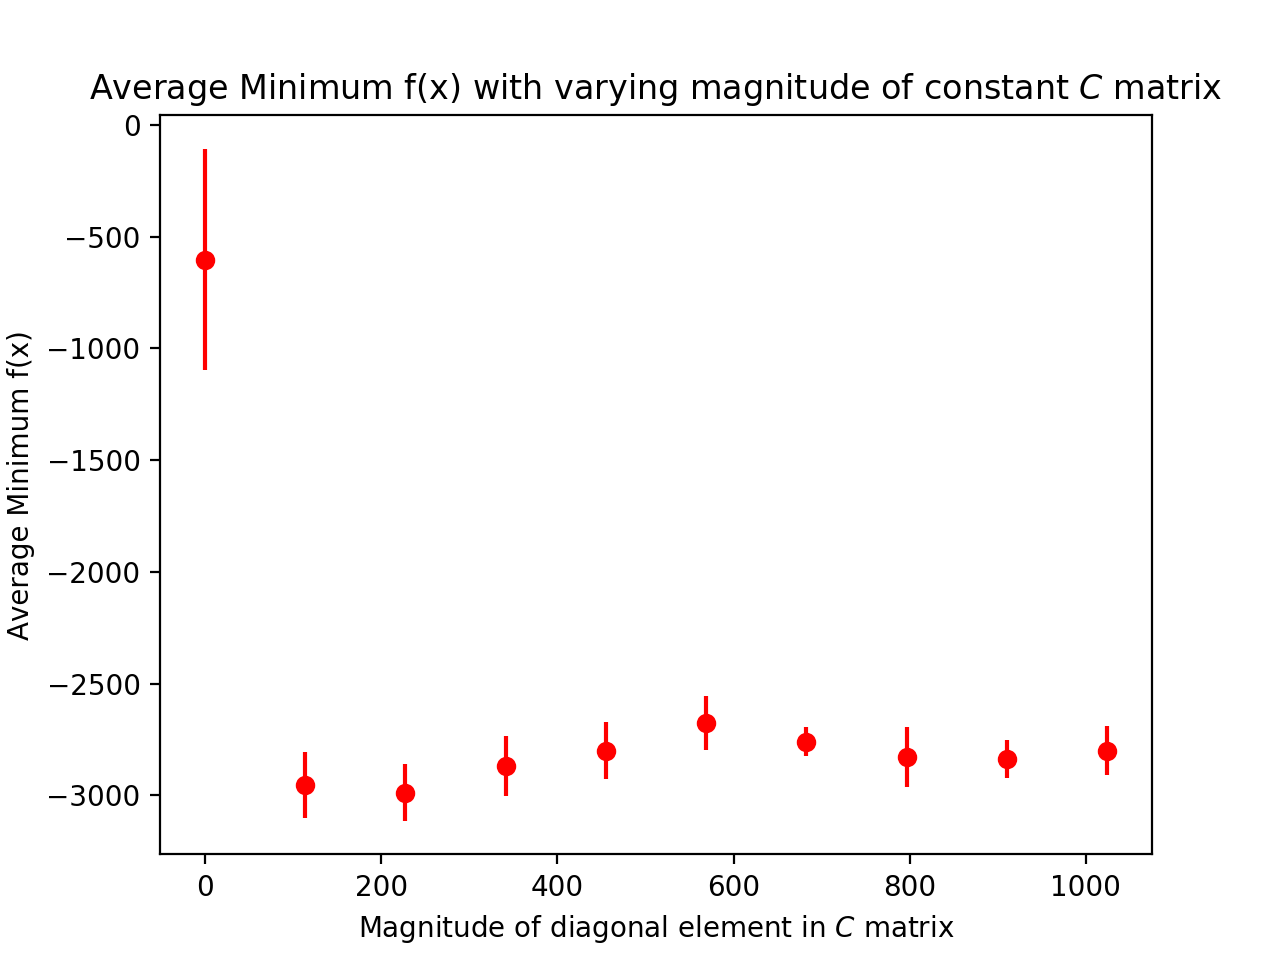
\includegraphics[width=8cm]{a_C_vary}
		\caption{Varying magnitude of constant C matrix}
		\end{subfigure}%
		\begin{subfigure}{8cm}
		\centering
		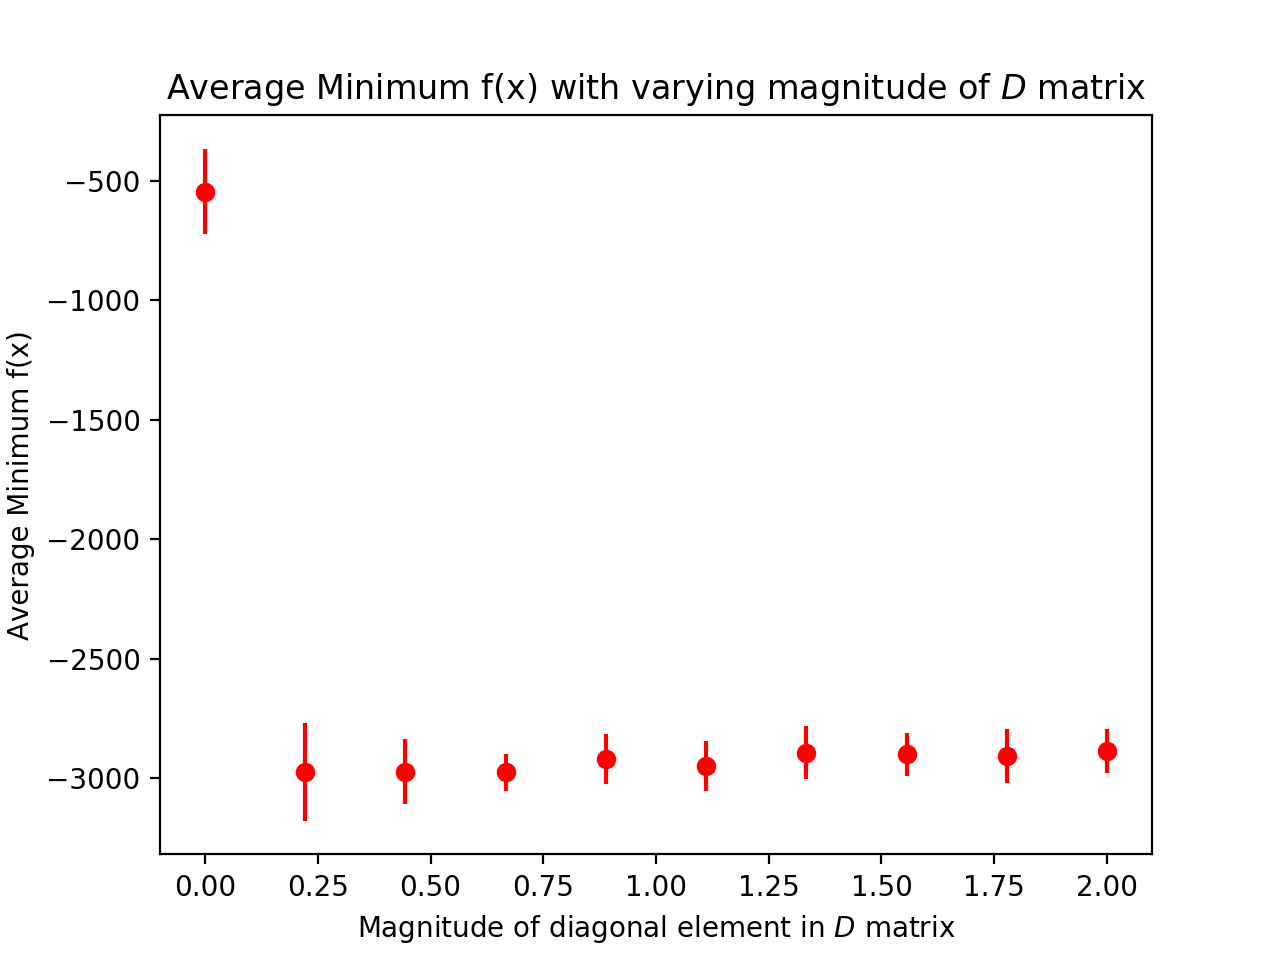
\includegraphics[width=8cm]{a_D_vary}
		\caption{Varying magnitude of variable D matrix}
		\end{subfigure}
		\caption{The effect of varying the magnitude of control variable update matrices on the average minimum f(x)}
		\label{fig8}
		\end{figure}
		\end{itemize}
		\pagebreak
		\item \textbf{Markov Chain Length}
		\begin{itemize}
		\item Temperatures are only updated at the end of each Markov Chain - a time set after either an arbitrary number of trials or alternatively, a threshold number of acceptances which is set to be proportional to the number of trials (as suggested in the notes).
		\item Thus, it might be expected that a longer Markov Chain might allow for more exploration of the space at the expense of being more likely to leave minima (because the probability of accepting an increase in objective function is higher).
		\item Meanwhile, a very small Markov chain will decrement T very quickly, meaning that the algorithm will most likely get stuck at a local minimum.
		\item I chose to test this by again looking at the average minimum objective function across 100 runs with a varying Markov Chain length. It was not worth using the actual minimum objective function across all runs because the values determined are highly stochastic do not depend nearly as much on the underlying structure of the algorithm.
		\item While there is a significant level of noise in the data (the standard deviations are very large), there is a certain trend as Markov Chains get larger: SA seems to perform more poorly with increase chain length (likely due to the reasons detailed above). 
		\item The algorithm seems to work best with small-sized chains - although the average minimum objective function value associated with the smallest chain is likely only small due to the fact that the burn-in implementation randomly finds and picks a starting sample that is most likely going to be in a local minima.	\begin{figure}[H]
		\centering
		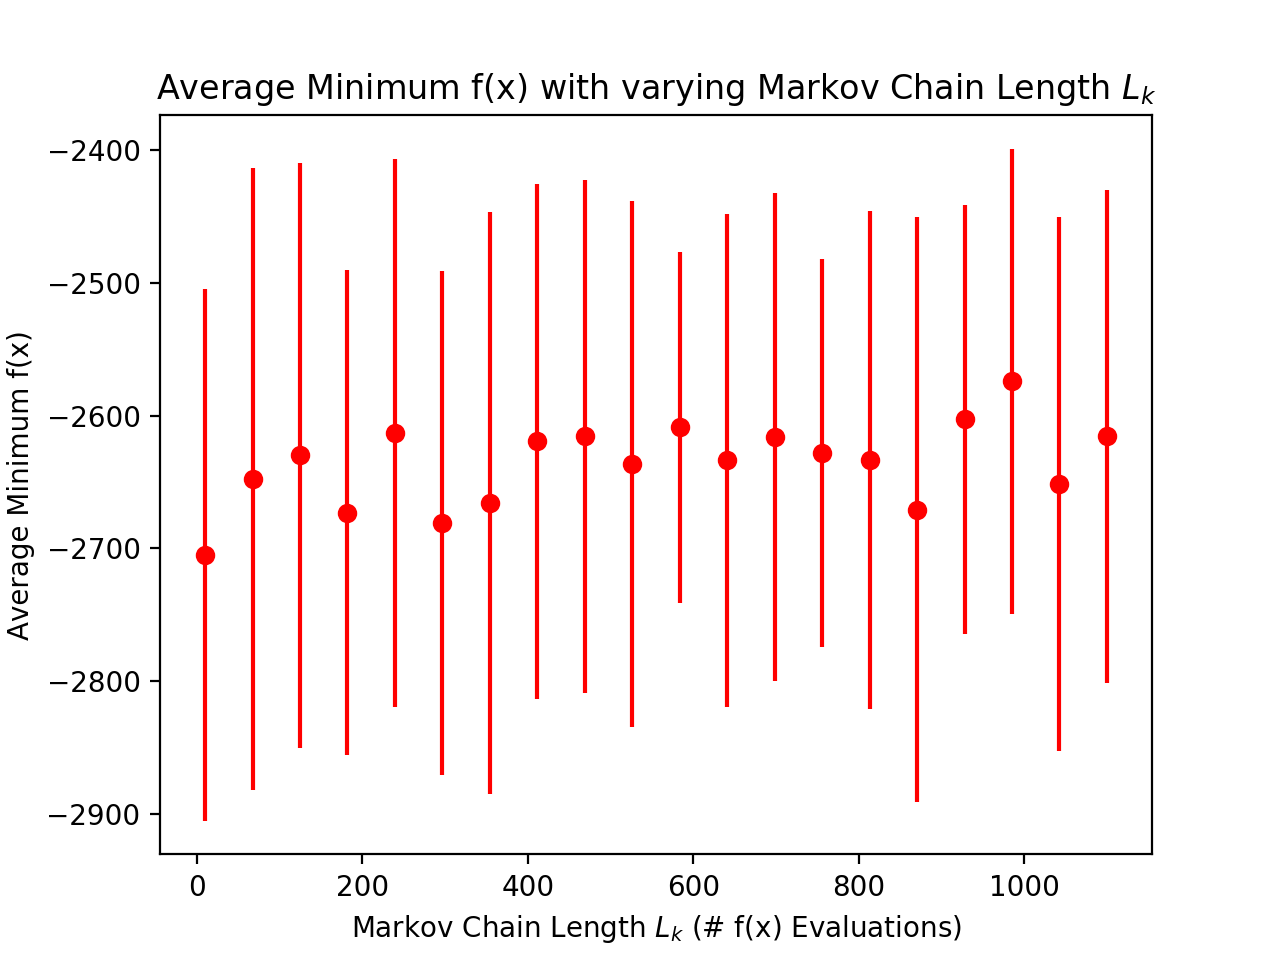
\includegraphics[width=9cm]{a_l_k}
		\caption{Average Minimum Objective Function with varying Markov Chain Length}
		\label{fig9}
		\end{figure}
		\end{itemize} 
		\pagebreak
		
		\end{itemize}
	\end{enumerate}
\end{enumerate}
\end{document}